\documentclass{article} % For LaTeX2e
\usepackage{nips13submit_e,times}
\usepackage{hyperref}
\usepackage{url}
\usepackage{graphicx}
\graphicspath{ {./} }
%\documentstyle[nips13submit_09,times,art10]{article} % For LaTeX 2.09


\title{Question Answering System with BiDAF and DCN}


\author{
Akshay Navalakha \\
\texttt{akshaynavalakha@gmail.com} \\
\And
Subin Modeel \\
\texttt{subin@apache.org} \\
}

% The \author macro works with any number of authors. There are two commands
% used to separate the names and addresses of multiple authors: \And and \AND.
%
% Using \And between authors leaves it to \LaTeX{} to determine where to break
% the lines. Using \AND forces a linebreak at that point. So, if \LaTeX{}
% puts 3 of 4 authors names on the first line, and the last on the second
% line, try using \AND instead of \And before the third author name.

\newcommand{\fix}{\marginpar{FIX}}
\newcommand{\new}{\marginpar{NEW}}

\nipsfinalcopy % Uncomment for camera-ready version

\begin{document}


\maketitle

\begin{abstract}
Machine comprehension (MC) is a challenging Natural Language Processing problem. It requires modelling the complex behaviour between the context and questions to find the answer. In this project, we have re-implemented from scratch two neural architecture for the QA task The Bidirectional Attention Flow
model(BiDAF) \& Dynamic Coattention Networks(DCN) with some modifications.We also experimented with using BiDAF decoder in DCN and DCN decoder in BiDAF.Our best model achieves an F1 score of  75.142\% F1 and 65.593\% EM on the test set with BiDAF model.
\end{abstract}

\section{Introduction}

Question answering (QA) is a task in natural language processing that requires both natural language understanding and world knowledge. In this task, a model must give answers to queries presented in natural language based on a context paragraph.The context contains the answer to the query. These problems require some attention mechanism between the context and the questions.

For the purposes of this project we use Stanford Question Answering dataset(SQUAD)[1] released by Rajpurkar et al. (2016). The SQUAD dataset is orders of magnitude larger than all previous hand-annotated datasets and has a variety of qualities that culminate in a natural QA task. SQuAD has the desirable quality that answers are spans in a reference document. This constrains answers to the space of all possible spans. However, Rajpurkar et al. (2016) show that the dataset retains a diverse set of answers and requires different forms of logical reasoning, including multi-sentence reasoning.

For the purpose of the paper we have explored a combination mainly from two neural architectures introduced in The Bidirectional Attention Flow model(BiDAF)[2] \& Dynamic Coattention Networks(DCN)[3].

In addition to re-implementing a vanilla BiDAF, we have experimented with substituting the output layer of the BiDAF with the Dynamic Pointer Decoder from the DCN paper. Also, in addition a bi-directional attention a self-attention layer (inspired from RNET) was inserted to get a BiDAF + Self Attention with a dynamic decoder network. A comparison in the performance of the three versions of BiDAF is shown in table 1 .

Apart from BiDAF, a Dynamic Coattention model  was re-implemented. Here we compute the affinity matrix between the context and question, which is then used to weight the continuous representations of the two documents.The decoder layer is complicated where it iteratively  estimates the start and end location of the answer, allowing it to better handle local minima. Two variants of the model were implemented one with decoder mentioned in the DCN paper, second one with BiDAF Decoder.


\section{Related Work}
The SQUAD is less than 2 years old but has led to significant amount of papers in reading comprehension. Wang \& Jiang (2016b) build question-aware passage representation with match-LSTM (Wang \& Jiang, 2016a), and predict
answer boundaries in the passage with pointer networks (Vinyals et al., 2015).  Seo et al. (2016) introduce bi-directional attention flow networks to model question-passage pairs at multiple levels of granularity. Xiong et al. (2016) propose dynamic co-attention networks which attend the question and passage simultaneously and iteratively refine answer. RNET(2018) uses gated attention between the question and context and self attention layer. These models have come very close to human performance. 

\section{Problem Statement}

Given a context words $( x^{Q}_{1} , x^{Q}_{2} , . . . , x^{Q}_{n} )$ denote words in the question and  $(x^{D}_{1} , x^{D}_{2} , . . . , x^{D}_{m} )$ we need to predict the answer span $(x_{s}, x_{e})$ from the context which matches answer to the question. A F1 and Exact match metric is used to evaluate the performance of the model. The squad dataset is divided into 80\%  training dataset, 10\% in dev dataset and 10\% in testing set (hidden).

\section{Dataset and Features}


We use pre-trained GloVe vectors  of 100 dimensional to represent the words in the context and question.Let \( x^{c}_{1} , x^{c}_{2} , . . . , x^{c}_{n} \)  denote word embedding in the context and \(x^{q}_{1} , x^{q}_{2} , . . . , x^{q}_{m} \) denote the same for words in the question. 
We found slight significant in performance when we increase dimensional of Glove vectors but that comes at the cost of increase in training time.So we use Glove vectors of 100 dimensional to conduct more experiments 

The lengths of answer, context and questions is plotted in fig 4 , fig 5 and fig 6 respectively. Based on the histogram output we decided to use a context length of 400 and question length of 30. Decreasing the context length from 600 to 400 led to a speedup of almost 2 times enabling us to run more number of experiments.


\section{Models}
In this section we describe the 2 different models and their variations. The first two models are re-implementation of the Bidaf without character level embedding[2] (referred to as vanilla BiDAF) and Dynamic Coattention network [3]. Then we interchanged the decoders of Bidaf and Co-attention to see the difference in performance resulting in what we refer to as Bidaf Dynamic.Replacing the decoder of the bidaf would provide it the flexibility of recovering local maxmima. The last two models is adding a self attention layer after the BiDAF attention layer in both vanilla Bidaf and Bidaf Dynamic. 

The description of the BIDAF with Self Attention and Dynamic Pointer and Dynamic Co-attention model is as below

\subsection{BiDAF with Self Attention and Dynamic Pointer}

We did a re-implementation of the BIDAF model without the character level encoding and added/ replaced some of the layers. The addition includes using a Iterative Decoder and a self attention mechanism as shown in fig 1.

\begin{figure}
\includegraphics[scale=.65]{template/Bidafselfdynamic.png}
\centering
\caption{BiDAF with Self Attention and Dynamic Pointer Decoder.}
\end{figure}

\subsubsection{Word Embedding Layer}
Maps each word in the context and questions to a vector space using a pre-trained word em- bedding model to produce \( x^{c}_{1} , x^{c}_{2} , . . . , x^{c}_{n} \)  words embedding for each word in  context and \(y^{q}_{1} , y^{q}_{2} , . . . , y^{q}_{m} \) word embedding for each word in questions

\subsubsection{RNN Encoder Layer}: 

The encoder is a bi-directional LSTM which is shared between the context and the questions. This gives us a better shared representation of the context and questions.
            $${c_1, . . . , c_N} = BiLSTM \{ x^{c}_{1} , x^{c}_{2} , . . . , x^{c}_{n}\} $$
            $${q_1, . . . , q_N} = BiLSTM \{ y^{q}_{1} , y^{q}_{2} , . . . , x^{c}_{n}\} $$

\subsubsection{Bidirectional Attention}
Couples the query and context vectors and produces a set of query- aware feature vectors for each word in the context.
Assume we have context hidden states $c_1, . . . , c_N \ \epsilon \  R^{2h} $ and question hidden states $q_1, . . . , q_M \ \epsilon \  R^{2h} $. We compute the similarity matrix $ S \ \epsilon \  R^{N\times M}$ , which contains a similarity score $S_{ij}$ for each pair $(c_i,q_j)$ of context and question hidden states.
$$S =w^{T}_{sim}[c_{i};q_{j};c_{i} o q_{j}]\ \epsilon \ R $$
Here, $c_{i} o q_{j} $ is an elementwise product and $ w_{sim} \ \epsilon \ R^{6h} $ is a weight vector.
Next, we perform Context-to-Question (C2Q) Attention. (This is similar to our baseline’s Attention Layer). We take the row-wise softmax of S to obtain attention distributions $ \alpha^i$, which we use to take weighted sums of the question hidden states $q_j$, yielding C2Q attention outputs $a_i$.
In equations, this is:
$$\alpha^i = softmax(S_i,:)\ \epsilon \ R^{M} \\     \forall i \ \epsilon \ \{1,...,N\} $$
$$a_i =  \sum_{j=1}^{M}\alpha^{i}_{j}q_j \ \epsilon \ R^{2h} \   \forall i\ \epsilon \ \{1,...,N \}$$
Next, we perform Question-to-Context(Q2C) Attention. For each context location $i\ \epsilon \ \{1,...,N \}$, we take the max of the corresponding row of the similarity matrix, $m_{i} = max_{j} S_{ij} \ \epsilon \ R$. Then we take the softmax over the resulting vector $m \ \epsilon \ R^{N} $ – this gives us an attention distribution $\beta \ \epsilon \ R^{N}$ over context locations. We then use $\beta$ to take a weighted sum of the context hidden states $c_{i}$ – this is the Q2C attention output $c^{'}$. In equations:
$$ m_{i} = max_{j}S_{ij} \ \epsilon \ R^{N} \forall i \ \epsilon \ \{1,...,N\}\ $$
$$ \beta = softmax(m)\ \epsilon \ R^N $$
$$c^{'} = \sum_{i=1}^{N}\beta_{i}c_{i} \ \epsilon \ R^{2h} $$

Lastly, for each context location $i \ \epsilon \ \{1,...,N\}$ we obtain the output $b_i$ of the Bidirectional Attention Flow Layer by combining the context hidden state $c_i$, the C2Q attention output $a_i$, and

the Q2C attention output c′:
$$b_{i} =[c_{i};a_{i};c_{i}oa_{i};c_{i} o c^{'}] \ \epsilon \ R^{8h} \forall i \ \epsilon \ \{1,...,N\}$$
where ◦ represents element-wise multiplication.


\subsubsection{Self Attention}
A self attention layer was inserted between the bi-directional layer and decoder. Even though LSTM should be able to theoretically capture the references between context of large length, practically it fails because of vanishing gradients. So a self-attention layer was introduced to relate the current word in the context with all other words.

The output of the bidirectional layer is feed into the self attention module.
$$e^{i}_{j} = tanh(W_{1}b_{j} + W_{2}b{i})$$
$$\alpha^{i} = softmax(e^{i})$$
$$a^{i} = \sum_{j=1}^{N}\alpha^{i}_{j}b_{j}$$

The output of the bidirectional layer and self attention are concatenated before sending it out to the modelling layer
$$H = [b; a]$$

\subsubsection{Modeling Layer}
We have kept the modelling layer the same as in the original BIDAF paper. It takes in H which is $R^{N x 16d}$, which encodes the query-aware representations concatenated with the self attention. This layer captures the interaction between the context and the query. We use a bi-directional LSTM of 2 layers with a ouptut size of d for each direction.




\subsubsection{Dynamic Answer Pointer}
The dynamic answer decoder is similar to the one used in DCN[3]. The output of the model layer is feed into the dynamic decoder. The initial state of the LSTM is all set to zero and the initial start and end word is selected to be the first word of the context. The decoder using a LSTM and a highway max network. The motivation of substituting the original decoder with the iterative reasoning decoder was that the model could recover from the local maxima. A improved performance of 1\% on F1 score was achieved after substituting the original decoder with the iterative reasoning decoder.
For the decoder the initial state for the start word and end word is set to the first context word. Also, the initial state of the LSTM is set to be zero valued tensor. It is expected that the model will learn from this init state and iteratively update the start and end word.


\subsection{DCN}

\subsubsection{Encoder}
We encode the Context as : $d_{t} = LSTM_{enc} \langle d_{t-1},x^{D}_{t} \rangle $ using a LSTM. 
We define the context encoding matrix as $ D = \langle d_{1} ...d_{m},d_{\emptyset} \rangle $ $ \ \epsilon \  R^{l\times(m+1)} $.
We also add a sentinel vector $ d_{\emptyset} $ (Merity et al., 2016), which we later show allows the model to not attend to any particular word in the input.

The question embeddings are computed with the same LSTM to share representation power: $ q_{t} =LSTM_{enc} \langle q_{t-1} , x^{Q}_{t} \rangle $ .
We define an intermediate question representation $ Q′ = \langle q_{1} . . . q_{n},q_{\emptyset} \rangle $ $ \ \epsilon \  R^{l\times(n+1)} $.
To allow for variation between the question encoding space and the document encod- ing space, we introduce a non-linear projection layer on top of the question encoding. 
The final representation for the question becomes: $ Q = tanh \langle   W^Q Q′ + b^Q \rangle \  \epsilon \  R^{l\times(n+1)} $

\begin{figure}
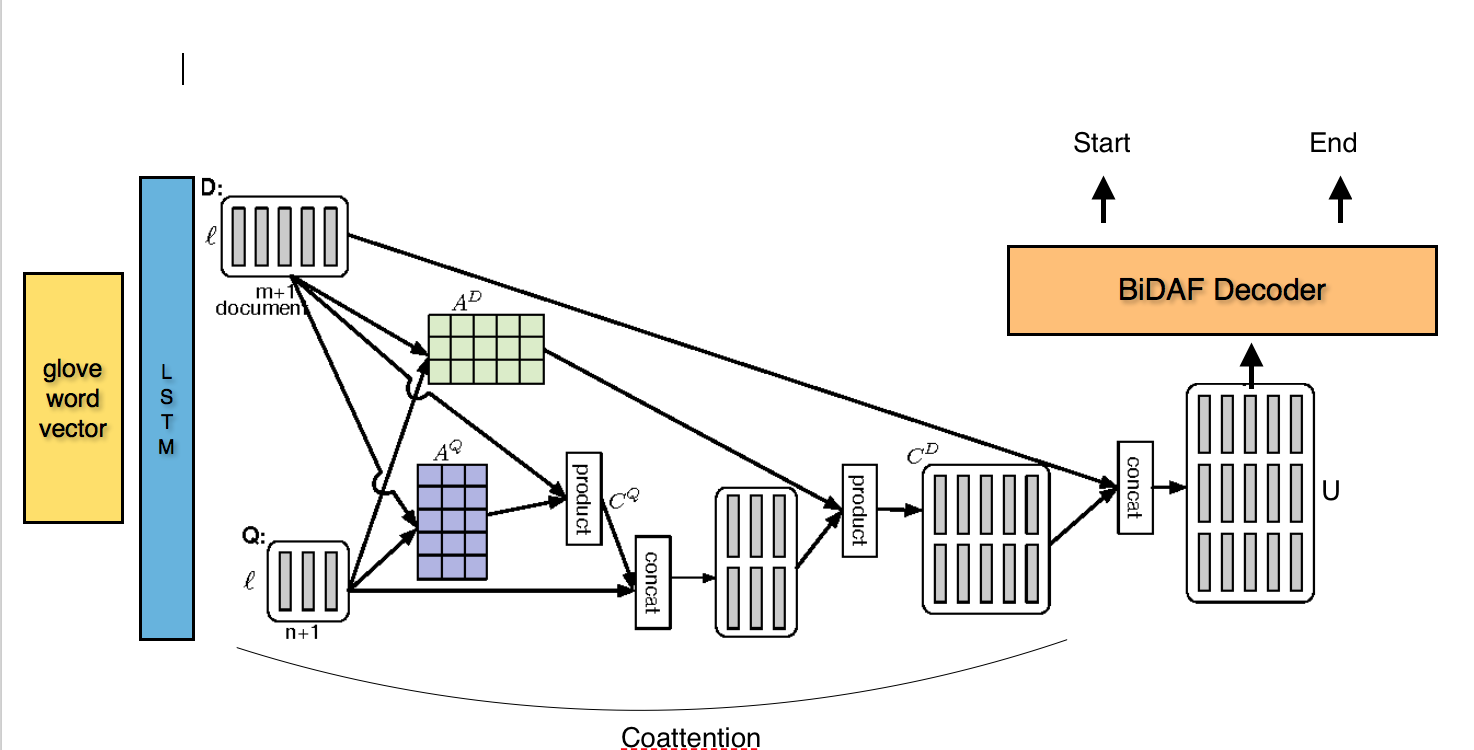
\includegraphics[scale=.5]{template/coatt_bidaf.png}
\centering
\caption{Coattention with BiDAF Decoder}
\end{figure}

\begin{figure}
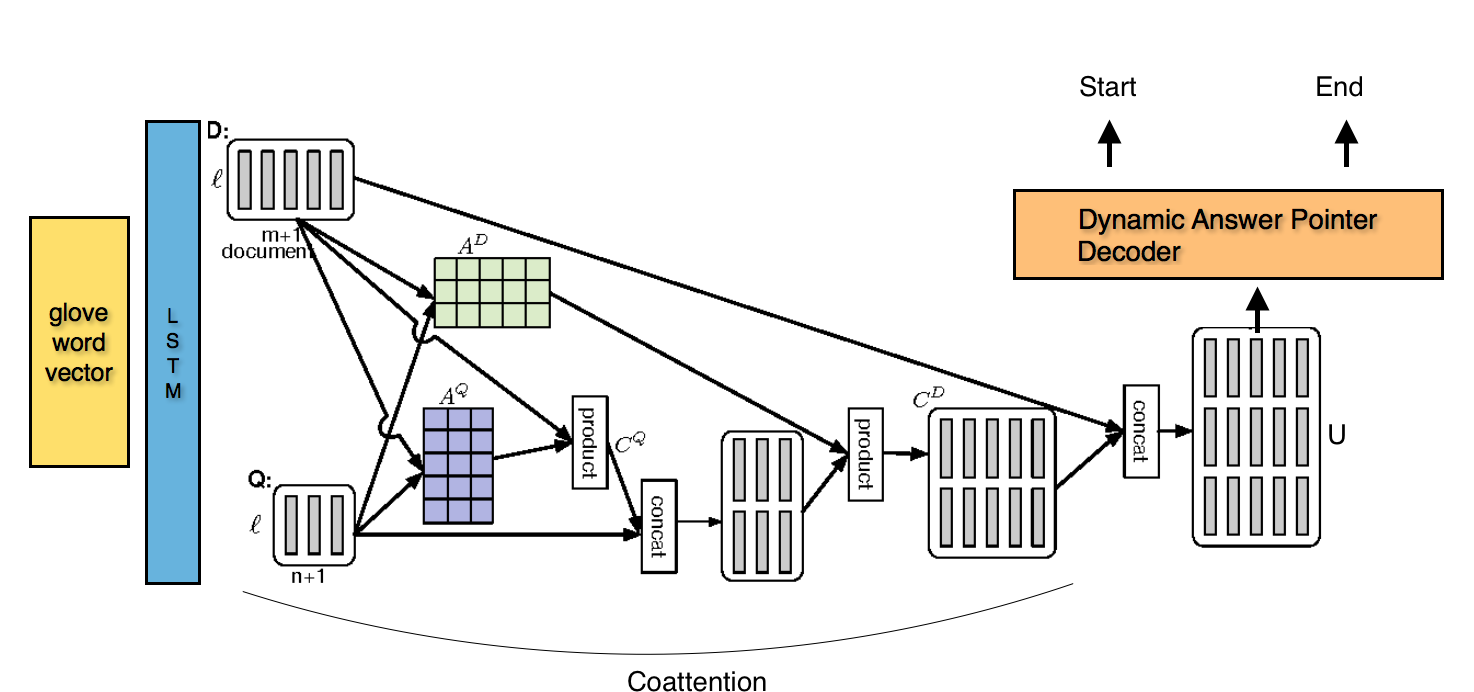
\includegraphics[scale=.5]{template/coatt_dynamic.png}
\centering
\caption{Coattention with Dynamic Pointer Decoder length distribution.}
\end{figure}

\subsubsection{Coattention}

The coattention mechanism  attends to the question and document simultaneously, similar to (Lu et al., 2016), and finally fuses both attention contexts. Figure 2 and Figure 3 provides an illustration of the coattention models we implemented.
We first compute the affinity matrix, which contains affinity scores corresponding to all pairs of document words and question words: $ L = D^{T}Q \ \epsilon \  R^{(m+1)\times(n+1)} $. The affinity matrix is nor-
malized row-wise to produce the attention weights $A^{Q}$ across the document for each word in the question, and column-wise to produce the attention weights $A^{D}$ across the question for each word in the document:
$$A^{Q} = softmax (L) \  \epsilon \ R^{(m+1)\times(n+1)} \ and \  A^{D} = softmax(L^{T}) \ \epsilon \ R^{(n+1)\times(m+1)}  $$
Next, we compute the summaries, or attention contexts, of the document in light of each word of the question.
$$C^{Q} = DA^{Q} \  \epsilon \  R^{l\times(n+1)}$$


We similarly compute the summaries $QA^{D}$ of the question in light of each word of the document. Similar to Cui et al. (2016), we also compute the summaries $C^{Q}A^{D}$ of the previous attention con- texts in light of each word of the document. These two operations can be done in parallel, as is shown in Eq. 3. One possible interpretation for the operation $C^{Q}A^{D}$ is the mapping of question encoding into space of document encodings.
$$C^{D} = [Q;C^{Q}] A^{D} \ \epsilon \ R^{2l\times(m+1)}$$. We define $C^{D}$, a co-dependent representation of the question and document, as the coattention
context. We use the notation $[a; b]$ for concatenating the vectors a and b horizontally.
The last step is the fusion of temporal information to the coattention context via a bidirectional
LSTM: $$
u_{t} = BiLSTM ( u_{t−1}, u_{t+1},  [d_{t}; c^{D}_{t}])    \ \epsilon \  R^{2l}.$$ We define $U =[u_1,...,u_m]\ \epsilon \ R^{2l \times m} $ ,which provides a foundation for selecting which span may
be the best possible answer, as the coattention encoding.

\subsubsection{Decoder}
We used a Dynamic Answer Pointer Decoder as mentioned in DCN and then we replaced that with a BiDAF Decoder.

\section{Experiments}
We found that most of the context were below 400.So we used context length 400 in our models.This reduced time taken to run our models.We tried to build different models and compare the improvements for each of the models.We see that moving from Co-attention to Bidaf gave us 3 \% points improvement on the dev leaderboard. Substituting the Bidaf decoder with the dynamic decoder gave an improved performance of 1\% on F1 score with a hidden size of 100. The best model which we got was for bidaf implementation with a bidaf decoder with a hidden size of 200. We could'nt test a hidden size of 200 with the dynamic decoder because of space constraints.

Table 1 gives a comparison of the different models performance. The best score of 75\% on FM score was achieved on the test score.

\begin{figure}
\minipage{0.32\textwidth}
  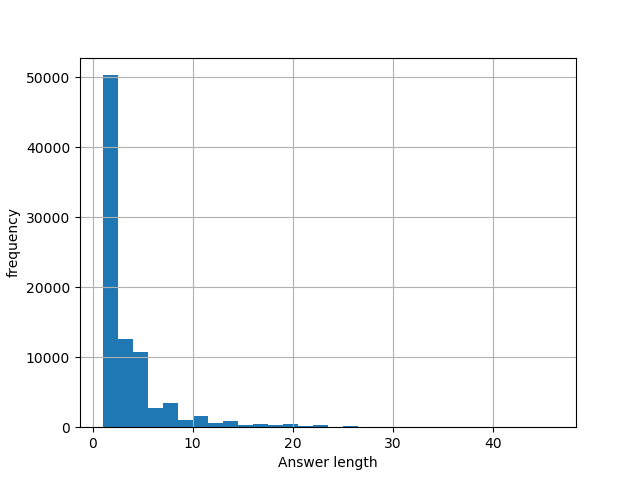
\includegraphics[width=\linewidth]{template/Answer.png}
  \caption{Answer length distribution.}
\endminipage\hfill
\minipage{0.32\textwidth}
  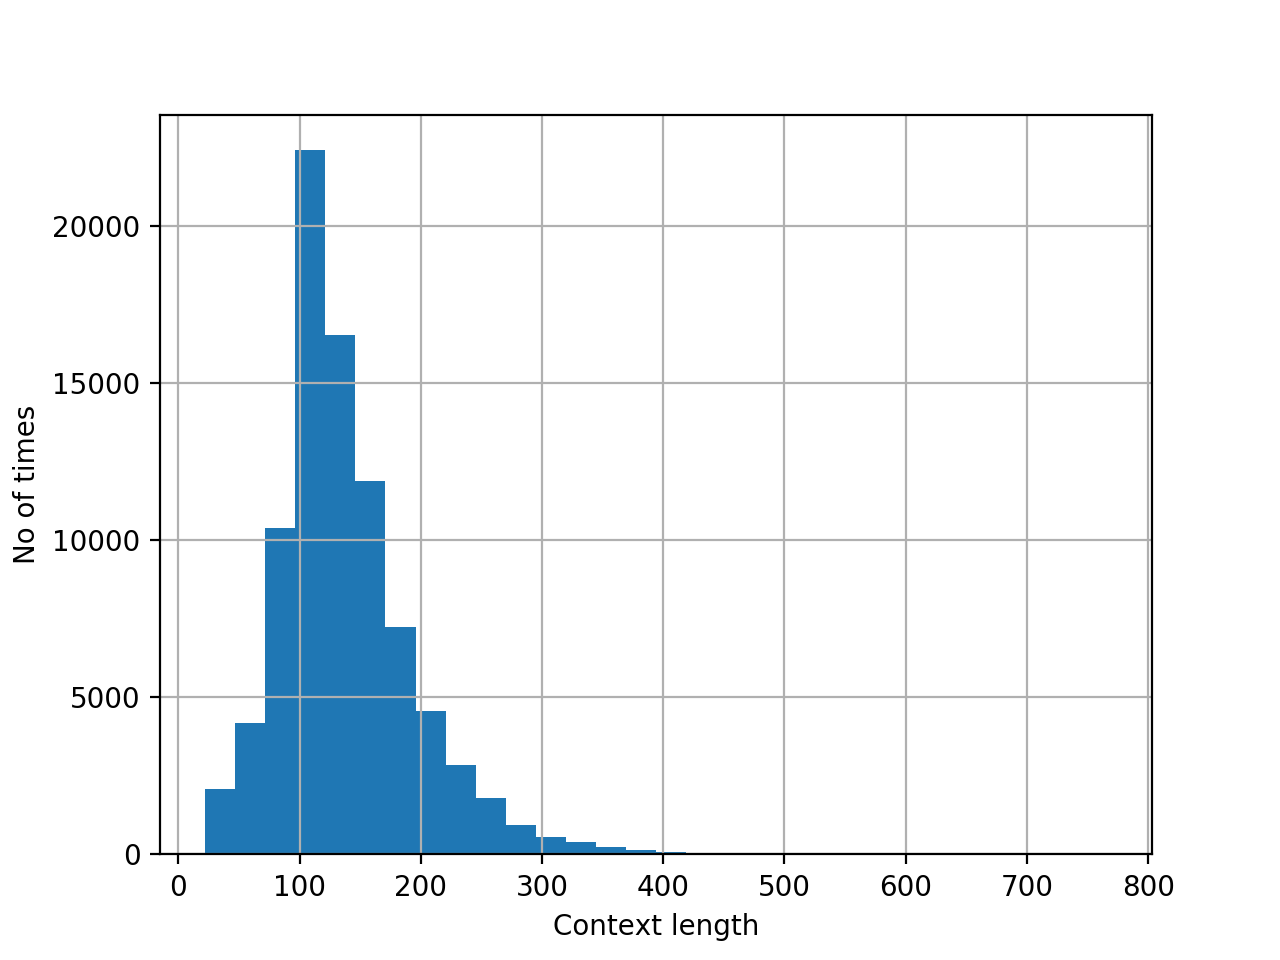
\includegraphics[width=\linewidth]{template/Context.png}
  \caption{Context length distribution.}
\endminipage\hfill
\minipage{0.32\textwidth}
  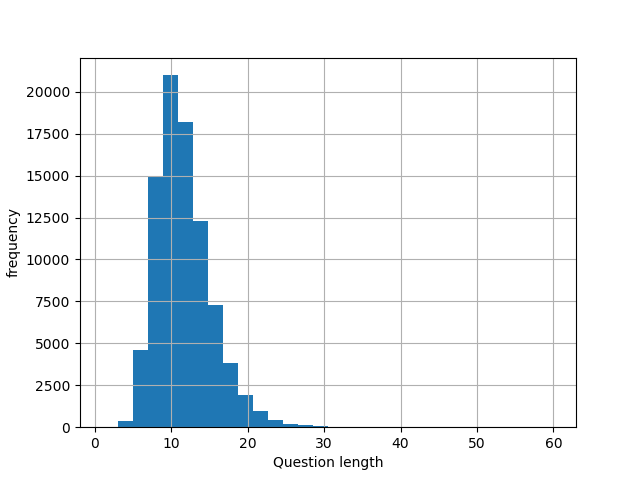
\includegraphics[width=\linewidth]{template/Question.png}
  \caption{Question length distribution.}
\endminipage\hfill
\end{figure}

\begin{figure}
\minipage{0.5\textwidth}
  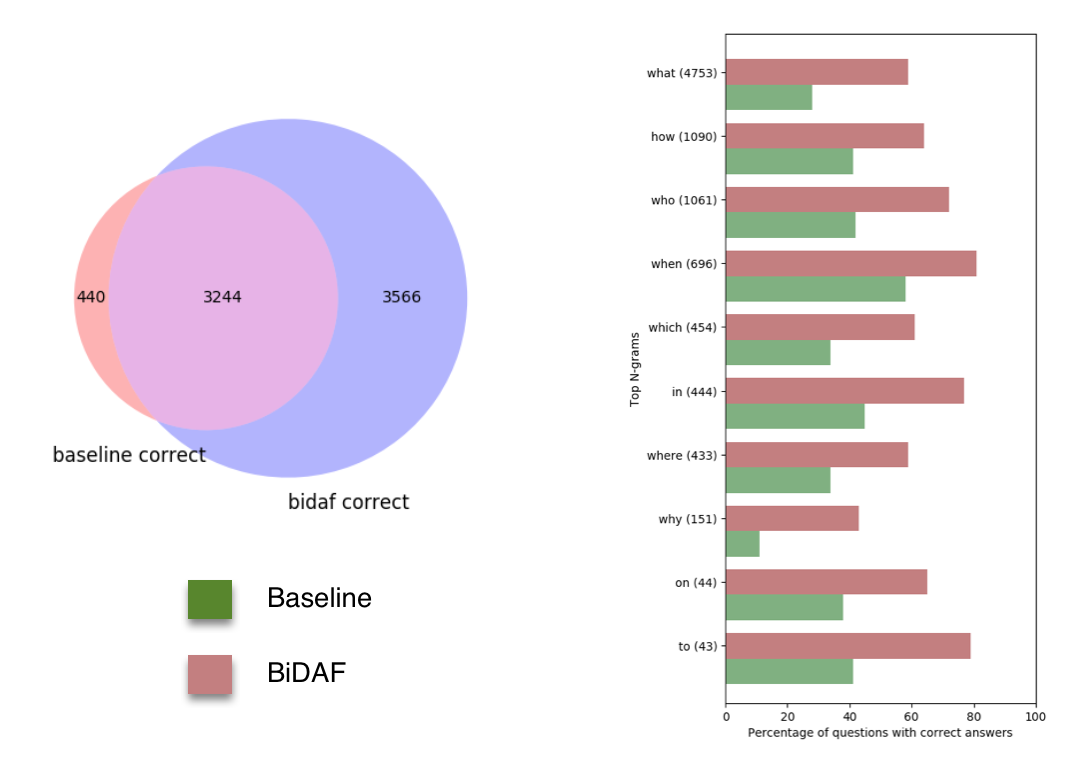
\includegraphics[width=\linewidth]{template/pie_baseline_bidaf.png}
\endminipage\hfill
\minipage{0.5\textwidth}
  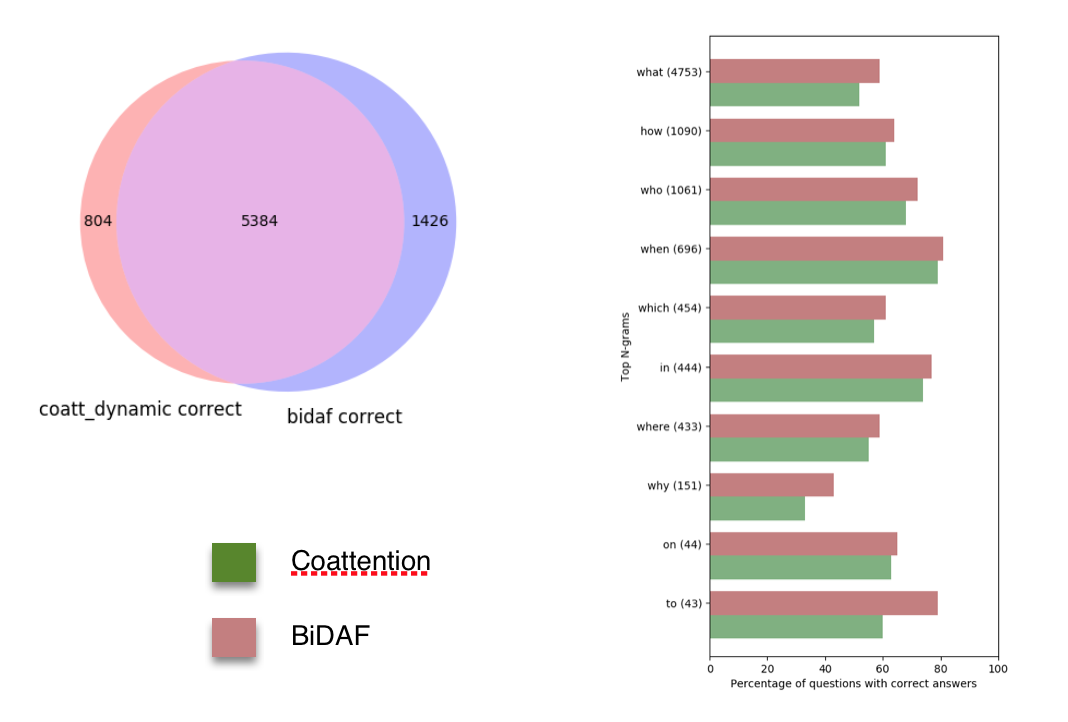
\includegraphics[width=\linewidth]{template/pie_coatt_bidaf.png}
\endminipage\hfill
\caption{Venn diagram of the questions answered correctly(i.e EM) by our models(total Q=10570).\& Correctly answered questions broken down by the 10 most frequent first words in the question}
\end{figure}

Adding the self-attention layer provided provided a slight improvement in performance.

To reduce the over-fitting problem we tried with dropouts ranging from 0.15 to 0.3 and regularization factor of 0.0001 to 0.001. It seems that the regularization and dropout had very little effect on the model and the dev loss begins to plateau off at or near dev F1 score of 68\%.

An experiment to understand the impact of learning rate was also performed. We changed the learning rate from 0.001 to 0.0001. As the learning rate decreases we get a smoother graph for the loss.



\begin{table}[ht]
\caption{Leaderboard Performance} % title of Table
\centering % used for centering table
\begin{tabular}{c c c c c} % centered columns (4 columns)
\hline\hline %inserts double horizontal lines
Model & Dev EM & Dev F1 & Test EM & Test F1 \\ [0.5ex] % inserts table
%heading
\hline % inserts single horizontal line
BiDAF Attention + BidaF decoder (Ours) & 64.427 & 74.444 & 65.593 & 75.142 \\
BiDAF Attention + Answer Pointer decoder (Ours) & 63.652 & 74.024 & 64.597 & 74.364 \\ 	
BiDAF Attention + Self Attention (Ours) & 63.500 & 73.638 & - & -\\
BiDAF Attention + Self Attention + Answer Pointer decoder (Ours) & 63.954 & 74.051 & - & -\\
\\ \hline \\
Coattention Only (Ours) & 53.955 & 64.171 & - & -\\
Coattention with BidaF decoder (Ours) & 58.079 & 69.008 & - & -\\
Coattention with Answer Pointer decoder (Ours) & 58.543 & 69.390 & - & -\\
\\ \hline \\
BiDAF & - & 76.3 & - & 76.9\\
DCN  & 65.4 & 75.6 & 66.2 & 75.9\\
SQUAD Baseline(Ours) & 34.853 & 44.117 & - & -\\
Human (Rajpurkar et al., 2016) & 81.4 & 91.0 & 82.3 & 91.2\\ [1ex] % [1ex] adds vertical space
\hline %inserts single line
\end{tabular}
\label{table:nonlin} % is used to refer this table in the text
\end{table}



 

\section{Conclusion}

We were able to build a good model for answering questions presented to it in natural language. Of the 4 models we developed our BiDAF model was able to achieve better performance.
As of right now, we achieve a F1 score of 75.142 and an EM score of 65.593 which is on par with some of the entries on the official SQuAD leaderboard.

\begin{figure}
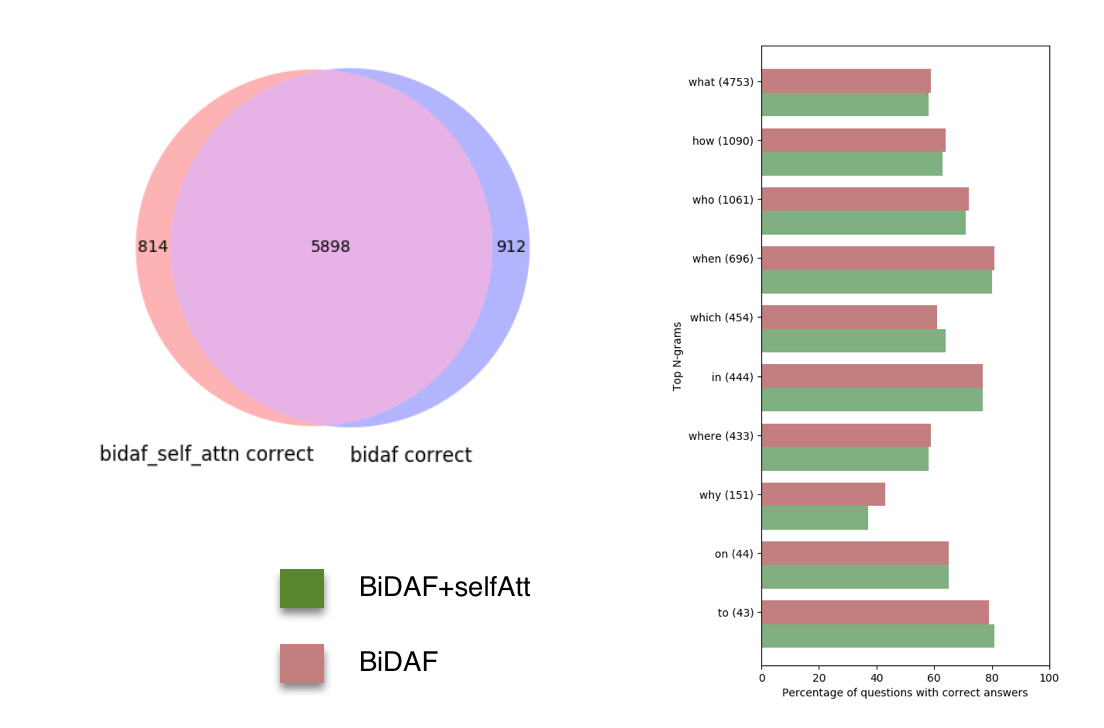
\includegraphics[scale=.5]{template/pie_bidaf_bidaf_self.png}
\centering
\caption{Venn diagram of the questions answered correctly(i.e EM) by our models(total Q=10570).\& Correctly answered questions broken down by the 10 most frequent first words in the question}
\end{figure}

\subsection*{Future Work}

There are a few more experiments we would like to try in the future like using more word features.
The original BiDAF implementation used character encoding which was not implemented by us and there is still scope for further hyperparameter tuning and bug fixing.
Coattention with self attention gave poor performace.We would like to implement DCP+[7] which is based on stacked coattention to improve performance Since Vaswani et al. (2017) show that the stacking of attention layers helps model long-range dependencies. We would also like to improve the performance of Coattention with Dynamic Pointer Decoder.




\section{Contribution}
The BIDAF model implementation, Dynamic Decoder from the Co-attention paper and Self Attention module was coded by Akshay.
The encoder and attention layer from DCN for Co-attention, and a simplified BiDAF decoder for Coattention was done by Subin.Subin wrote scripts for visualizations.

\section{Acknowledgments}

We would like to thank Richard Socher, and all the TAs for this course.
We would also like to give our thanks to Microsoft for providing GPUs on Azure to train our models.

\section*{References}

\small{

[1] P. Rajpurkar, J. Zhang, K. Lopyrev, and P. Liang, “Squad: 100,000+ questions for machine comprehension of text,” arXiv preprint \href{https://arxiv.org/abs/1606.05250}{arXiv:1606.05250}, 2016.

[2] M. Seo, A. Kembhavi, A. Farhadi, and H. Hajishirzi, “Bidirectional attention flow for machine comprehension,” arXiv preprint \href{https://arxiv.org/abs/1611.01603}{arXiv:1611.01603}, 2016.

[3] C. Xiong, V. Zhong, and R. Socher, “Dynamic coattention networks for question answering,” arXiv preprint \href{https://arxiv.org/abs/1611.01604}{arXiv:1611.01604}, 2016.

[4] J. Pennington, R. Socher, and C. D. Manning, “Glove: Global vectors for word representation.,” in EMNLP, vol. 14,\href{https://nlp.stanford.edu/pubs/glove.pdf}{pp. 1532–1543}, 2014.

[5] Ashish Vaswani, Noam Shazeer, Niki Parmar, Jakob Uszkoreit, Llion Jones, Aidan N. Gomez,
Lukasz Kaiser, and Illia Polosukhin. Attention is all you need. In NIPS, 2017.

[6]Rupesh Kumar Srivastava, Klaus Greff, Jurgen Schmidhuber. Highway Networks 	arXiv:1505.00387 2015.

[7]Caiming Xiong, Victor Zhong, Richard Socher ,DCN+: Mixed Objective and Deep Residual Coattention for Question Answering 	arXiv:1711.00106.
}

\end{document}
